\subsection{Measurements in the Past}

ATGC parameters of $WW\gamma$ vertex can be probed in $W\gamma$, $WW$, and $WZ$ measurements. Limits on $\Delta \kappa_\gamma$ and $\lambda_\gamma$ constants from different D0 \cite{ref_D0_aTGC_comb}, LEP \cite{ref_LEP_aTGC_comb}, ATLAS \cite{ref_7TeV_ATLAS}, \cite{ref_ATLAS_WW_8TeV}, \cite{ref_ATLAS_VW_8TeV} and CMS \cite{ref_7TeV_CMS}, \cite{ref_CMS_WW_7TeV}, \cite{ref_CMS_WW_8TeV}, \cite{ref_CMS_VW_7TeV} measurements are summarized in Fig.~\ref{fig:aTGC_cg}.\\ 

\begin{figure}[htb]
  \begin{center}
    {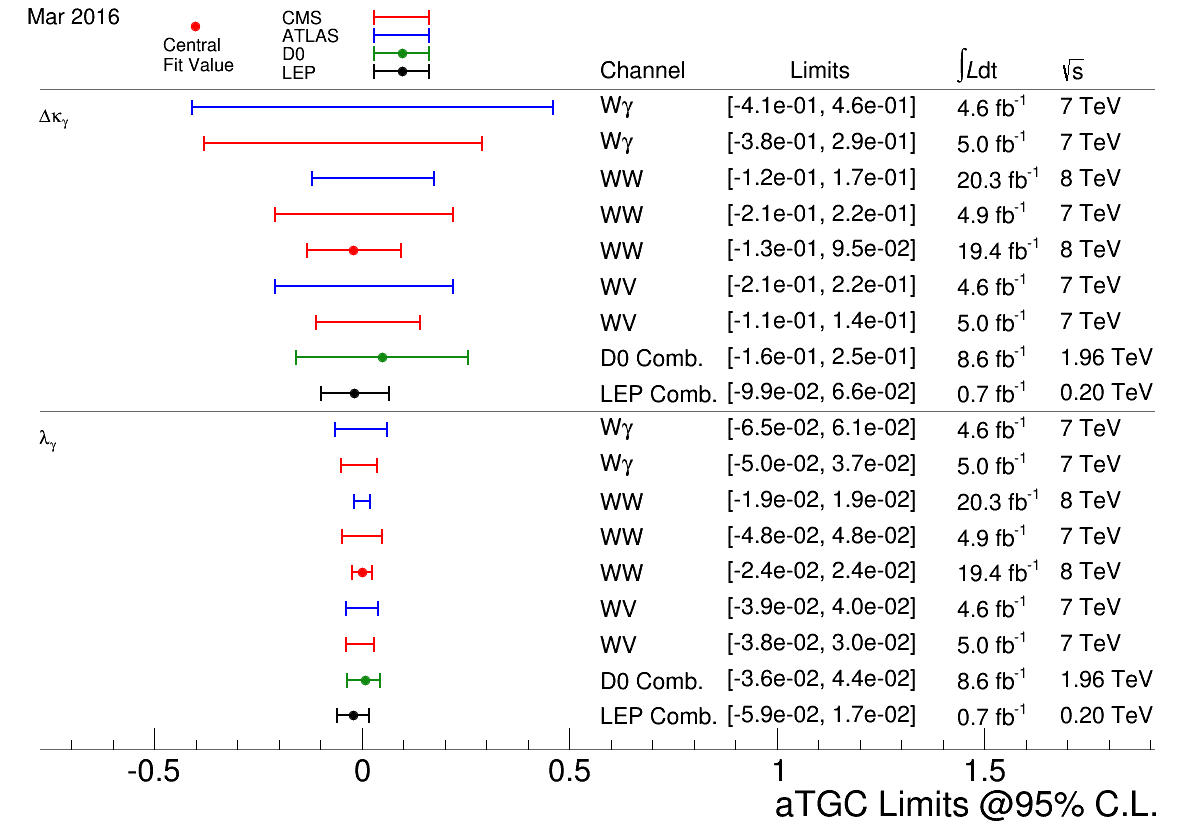
\includegraphics[width=0.80\textwidth]{../figs/WgAbout/aTGC_cg.png}}
    \caption{Summary of limits on the $WW\gamma$ aTGC coupling constants. Figure from \cite{ref_twiki_SMP_ATGC}}
    \label{fig:aTGC_cg}
  \end{center}
\end{figure}

The most recent measurements of $W\gamma$ production were performed by CMS \cite{ref_7TeV_CMS} and ATLAS \cite{ref_7TeV_ATLAS} collaborations with $pp$ collisions at $\sqrt{s}=7$~GeV collected in 2011. The measurements are based on~5~fb$^-1$ and~4.6~fb$^-1$ of integrated luminosity with CMS and ATLAS respectively. Both collaborations considered two channels: $W\gamma\rightarrow\mu\nu\gamma$ and $W\gamma\rightarrow e\nu\gamma$.\\

The $p_T^\gamma$ spectra of the selected events in data superimposed with selected events in the simulation of the signal and estimated background contribution for the muon and electron channels are shown in Fig.~\ref{fig:Wg7TeV_CMS_ptGamma} for CMS and in Fig.~\ref{fig:Wg7TeV_ATLAS_ptGamma} for ATLAS. \\

The major source of the background is the fake photon background where hadronic jets are misidentified as photons. Such events originate from $W+$jets process mostly but $Z+$jets and $\bar{t}t+$jets events contribute to this source of the background as well. The second major background for the electron channel is the fake photon background where electron can be misidentified as a photon.  Such events are coming from $Z+$jets events. Other sources of backgrounds include real-$\gamma$ backgrounds, fake lepton + real photon and fake lepton + fake photon sources. Fig.~\ref{fig:Wg7TeV_CMS_ptGamma} and Fig.~\ref{fig:Wg7TeV_ATLAS_ptGamma} show a good agreement.\\

\begin{figure}[htb]
  \begin{center}
    {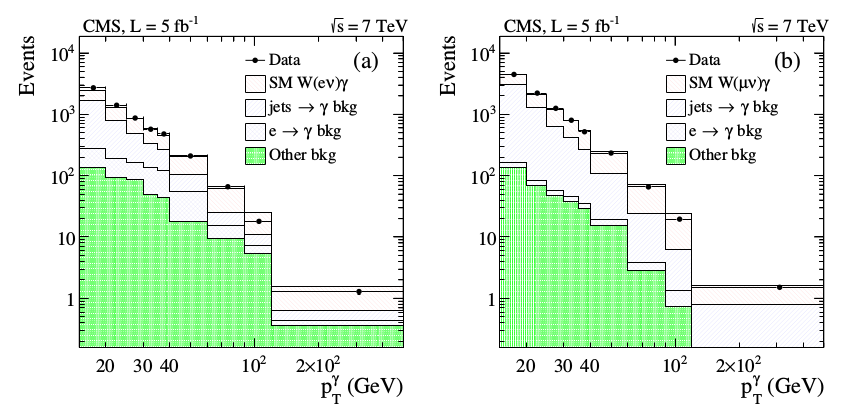
\includegraphics[width=0.80\textwidth]{../figs/WgAbout/Wg7TeV_CMS_ptGamma.png}}
    \caption{The distribution fo the $p_T^\gamma$ of W$\gamma$ candidates in the analysis of 7 TeV CMS data. Data vs signal MC + background estimates. Left: $W\gamma\rightarrow e\nu\gamma$, right: $W\gamma\rightarrow \mu\nu\gamma$ \cite{ref_7TeV_CMS}.}
    \label{fig:Wg7TeV_CMS_ptGamma}
  \end{center}
\end{figure}

\begin{figure}[htb]
  \begin{center}
    {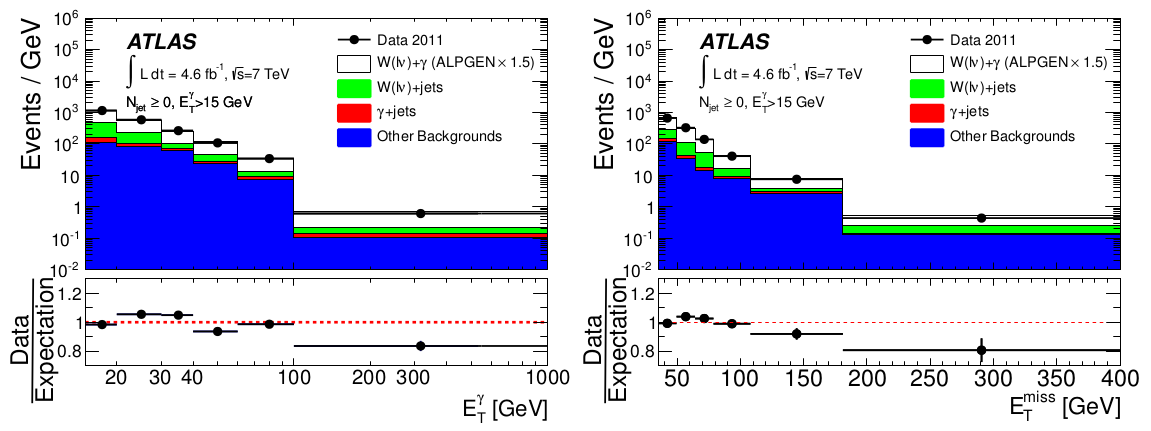
\includegraphics[width=0.80\textwidth]{../figs/WgAbout/Wg7TeV_ATLAS_ptGamma.png}}
    \caption{The distribution fo the $p_T^\gamma$ (left) and $E_T^\gamma$ (right) of W$\gamma$ candidates in the analysis of 7 TeV ATLAS data. Data vs signal MC + background estimates \cite{ref_7TeV_ATLAS}. }
    \label{fig:Wg7TeV_ATLAS_ptGamma}
  \end{center}
\end{figure}

CMS provides measurements of the $P_T^\gamma$ spectrum, the total cross section within the phase spaces of $\Delta R>0.7$, $P_T^\gamma>15$~GeV, $P_T^\gamma>60$~GeV and $P_T^\gamma>90$~GeV, and limits on aTGC coupling constants.\\

ATLAS, in addition to the $P_T^\gamma$ spectrum, total cross section and limits, provides the differential cross section and cross section with different number of associated jets. No evidence of a new physics is observed.\\


